\chapter{Modelo de Negocio\index{Negocio}}
\label{chap:Negocio}
\textit{En el presente capítulo se despliega el desarrollo de la Arquitectura Empresarial\index{Arquitectura Empresarial} correspondiente al Modelo de Negocio\index{Negocio} utilizando Archimate\index{Archimate}.}
\vspace{2ex}\vfill
\minitoc
\newpage

\section{Punto de Vista de la Organización\index{Organización}}
 El punto de vista de la organización se enfoca en el interior de la organización, un departamento, una red de empresas, es un punto de vista muy útil ya que permite identificar  competencias, autoridad y responsabilidades en una organización. \cite{ref9}
 
  \begin{table}[H]
	\centering
	\begin{tabular}{p{3.7cm}p{8cm}}
		\hline
		\rowcolor[HTML]{0073a1}
		{\color[HTML]{FFFFFF} \textbf{Nombre}} & {\color[HTML]{FFFFFF} \textbf{Organización\index{Organización}}} \\
		\hline
		\textbf{Stakeholder\index{Stakeholder}s} & Organización\index{Organización}, arquitectos de dominio y proceso, gerentes, empleados, accionistas \\
		\textbf{Preocupaciones} & Identificación de competencias, autoridad y responsabilidades \\
		\textbf{Propósito} & Diseñar\index{Diseñar}, decidir, informar \\
		\textbf{Nivel de Abstracción\index{Abstracción}} & Coherencia\index{Coherencia} \\
		\textbf{Capa} & Capa de negocio \\
		\textbf{Aspectos} & Activo \\
		\bottomrule
	\end{tabular}
	\captionsetup{width=.95\textwidth}
	\caption{Descripción Punto de Vista de la Organización\index{Organización} \cite{ref9}}
	\label{tabla4}
  \end{table}

  \begin{figure}[H]
 	\centering
 	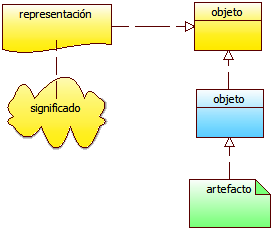
\includegraphics[scale=0.2]{figuras/14}
 	\captionsetup{width=.95\textwidth}
 	\caption{Posición del punto de vista de organización conceptualmente y marco del punto de vista \cite{ref9}}
 	\label{figura14}
  \end{figure}

  \subsection{Metamodelo\index{Metamodelo}}
  En la Figura \ref{metamodelo1} se ilustra el metamodelo perteneciente al punto de vista de organización, el cual está compuesto de los conceptos de actor, rol, interface, colaboración y localización. En este punto de vista se destaca como concepto fundamental que el actor juega un rol el cual está ubicado en una localización haciendo parte de una colaboración de negocio y se comunica con su entorno a través de una interface. \cite{ref9}
 
 \begin{figure}[H]
   \centering
   \includegraphics{metamodelos/1}
   \captionsetup{width=.95\textwidth}
   \caption{Metamodelo\index{Metamodelo} Punto de vista organización \cite{ref9}}
   \label{metamodelo1}
 \end{figure}

 \subsection{Modelo mInstituto}
 Esta vista es la interpretación sobre el organigrama en donde se representan los roles desempeñados en la empresa para el proceso de Minstituto\index{Minstituto}, cabe resaltar la importancia de identificar los roles de la estructura organizacional y su interacción que permitirá establecer las estrategias necesarias para controlar los procesos.  Como actores se reconoce al desarrollador, el analista de pruebas y el ejecutivo comercial.
  \begin{figure}[H]
   \centering
   \includegraphics[scale=0.8]{modelos/1}
   \captionsetup{width=.95\textwidth}
   \caption{Modelo Punto de vista organización: minstituto}
   \label{modelo1}
  \end{figure}
  
  \section{Punto de Vista Cooperación\index{Cooperación} de Actor}
  Este punto de vista se enfoca en los actores y sus relaciones con el entorno que los cobija, es un punto de vista donde los Stakeholder\index{Stakeholder}s o interesados son la organización, los procesos y los arquitectos de dominio. La finalidad u objetivo de este punto de vista es la de diseñar, decidir e informar. \cite{ref9}
  
  \begin{table}[H]
  	\centering
  	\begin{tabular}{p{3.7cm}p{8cm}}
  		\hline
  		\rowcolor[HTML]{0073a1}
  		{\color[HTML]{FFFFFF} \textbf{Nombre}} & {\color[HTML]{FFFFFF} \textbf{Cooperación\index{Cooperación} de Actor}} \\
  		\hline
  		\textbf{Stakeholder\index{Stakeholder}s} & Organización\index{Organización}, arquitectos de dominio y proceso \\
  		\textbf{Preocupaciones} & Relación de actores con el entorno \\
  		\textbf{Propósito} & Diseñar\index{Diseñar}, decidir, informar \\
  		\textbf{Nivel de Abstracción\index{Abstracción}} & Detalle \\
  		\textbf{Capa} & Capa de negocio \\
  		\textbf{Aspectos} & Estructura\index{Estructura} Activa, Comportamiento\index{Comportamiento} \\
  		\bottomrule
  	\end{tabular}
  	\captionsetup{width=.95\textwidth}
  	\caption{Descripción Punto de Vista Cooperación\index{Cooperación} de Actor \cite{ref9}}
  	\label{tabla5}
  \end{table}
  
   \begin{figure}[H]
   	\centering
   	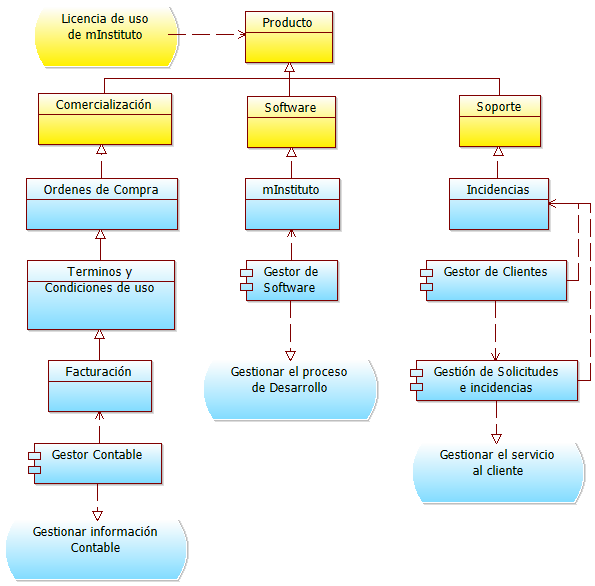
\includegraphics[scale=0.2]{figuras/15}
   	\captionsetup{width=.95\textwidth}
   	\caption{Posición del punto de vista cooperación de actor conceptualmente y marco del punto de vista \cite{ref9}}
   	\label{figura15}
   \end{figure}
  
  \subsection{Metamodelo\index{Metamodelo}}
  En la Figura \ref{metamodelo2} se ilustra el metamodelo perteneciente al punto de vista de cooperación de actor el cual esta compuesto de los conceptos de actor, rol, interface, colaboración, servicio de negocio, servicio de aplicación, interface de comunicación de aplicación y componentes de aplicación.\\
  
  En este punto de vista a el actor se le asigna un rol, el rol se compone de interfaces, a la interface se le asigna servicios y estos servicios van a una capa de aplicación a través de una interface que está conformada por componentes de aplicación y es usada por componentes de aplicación. \\
  
  Otro uso importante del punto de vista de cooperación de actor es mostrar como un número de actores de negocio cooperantes y / o componentes de aplicación juntos realizan un proceso de negocio. Por lo tanto, en esta vista, tanto actores de negocio como roles y componentes de aplicación pueden aparecer. \cite{ref9}
  
  \begin{figure}[H]
  	\centering
  	\includegraphics{metamodelos/2}
  	\captionsetup{width=.95\textwidth}
  	\caption{Metamodelo\index{Metamodelo} Punto de Vista Cooperación\index{Cooperación} de Actor \cite{ref9}}
  	\label{metamodelo2}
  \end{figure}
  
  \subsection{Modelo mInstituto}
  Para la empresa se establece una clara interacción por parte del área comercial con el cliente y retroalimentación para el equipo de proyecto, el cual se compone del área de producción, es decir, el desarrollador y el analista de pruebas, que serán los encargados de dar trámite a las solicitudes y requerimientos del cliente.
  
  \begin{figure}[H]
  	\centering
  	\includegraphics[scale=0.8]{modelos/2}
  	\captionsetup{width=.95\textwidth}
  	\caption{Modelo Punto de Vista Cooperación\index{Cooperación} de Actor: minstituto}
  	\label{modelo2}
  \end{figure}
 
  \section{Punto de Vista Función de Negocio\index{Negocio}}
  En este punto de vista se muestran las principales funciones de negocio de la organización y sus relaciones en términos de los flujos de información, valor, o productos entre ellas, los Stakeholder\index{Stakeholder}s o interesados son los procesos y arquitectos de dominio, administradores operacionales, tiene especial cuidado en la estructura de los procesos de negocio, su coherencia, integridad y las responsabilidades. \cite{ref9}

  \begin{table}[H]
  	\centering
  	\begin{tabular}{p{3.7cm}p{8cm}}
  		\hline
  		\rowcolor[HTML]{0073a1}
  		{\color[HTML]{FFFFFF} \textbf{Nombre}} & {\color[HTML]{FFFFFF} \textbf{Función de Negocio\index{Negocio}}} \\
  		\hline
  		\textbf{Stakeholder\index{Stakeholder}s} & Organización\index{Organización}, arquitectos de dominio y proceso \\
  		\textbf{Preocupaciones} & Identificación de competencias, identificación de actividades principales, reducción de la complejidad \\
  		\textbf{Propósito} & Diseñar\index{Diseñar} \\
  		\textbf{Nivel de Abstracción\index{Abstracción}} & Coherencia\index{Coherencia} \\
  		\textbf{Capa} & Capa de negocio \\
  		\textbf{Aspectos} & Comportamiento\index{Comportamiento} (Activo) \\
  		\bottomrule
  	\end{tabular}
   	\captionsetup{width=.95\textwidth}
   	\caption{Descripción Punto de Vista Función de Negocio\index{Negocio} \cite{ref9}}
   	\label{Tab:tabla6}
  \end{table}

  \begin{figure}[H]
   	\centering
   	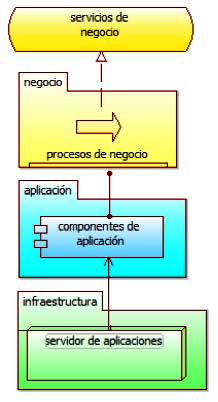
\includegraphics[scale=0.2]{figuras/16}
   	\captionsetup{width=.95\textwidth}
   	\caption{Posición del punto de vista función de negocio conceptualmente y marco del punto de vista \cite{ref9}}
   	\label{figura16}
   \end{figure}
    
   \subsection{Metamodelo\index{Metamodelo}}
   La Figura \ref{metamodelo3} muestra los conceptos de actor, rol y función; aquí se asignan tareas o funciones a estos actores, en el modelo se extrae lo que interesa, lo que se quiere capturar o tener en la mente. En este metamodelo aparecen dos tipos de relaciones el flujo y los disparos. \cite{ref9}
    
   \begin{figure}[H]
   	\centering
   	\includegraphics{metamodelos/3}
   	\captionsetup{width=.95\textwidth}
   	\caption{Metamodelo\index{Metamodelo} Punto de Vista Función de Negocio\index{Negocio} \cite{ref9}}
   	\label{metamodelo3}
   \end{figure}
    
    \subsection{Modelo mInstituto}
    En la vista se especifica la función principal de negocio la cual es la comercialización de licencias de uso del software a través de la captación de clientes por medio de material publicitario y la información que se presenta en el portal empresarial, la cual ha sido desarrollada por el diseñador.
    
    \begin{figure}[H]
    	\centering
    	\includegraphics[scale=0.75]{modelos/3}
    	\captionsetup{width=.95\textwidth}
    	\caption{Modelo Punto de Vista Función de Negocio\index{Negocio}: minstituto}
    	\label{modelo3}
    \end{figure}

  \section{Punto de Vista Proceso\index{Proceso} de Negocio\index{Negocio}}
  El punto de vista de proceso de negocio es el encargado de mostrar una estructura de alto nivel y composición de uno o más procesos de negocio. Tiene una complejidad importante, se incorporan elementos de comportamiento se incluye el proceso y/o función de negocio como elemento central, el proceso y/o función de negocio se ve afectado por las mismas relaciones con los demás conceptos, este punto de vista llama la atención en que nos induce a las entrañas de las organizaciones porque se ve lo que ellas hacen. \cite{ref9}
  
  \begin{table}[H]
  	\centering
  	\begin{tabular}{p{3.7cm}p{8cm}}
  		\hline
  		\rowcolor[HTML]{0073a1}
  		{\color[HTML]{FFFFFF} \textbf{Nombre}} & {\color[HTML]{FFFFFF} \textbf{Proceso\index{Proceso} de Negocio\index{Negocio}}} \\
  		\hline
  		\textbf{Stakeholder\index{Stakeholder}s} & Arquitectura de dominio y proceso, Gerentes de operación \\
  		\textbf{Preocupaciones} & Estructura\index{Estructura}r los procesos del negocio, consistencia, integridad y responsabilidades \\
  		\textbf{Propósito} & Diseñar\index{Diseñar} \\
  		\textbf{Nivel de Abstracción\index{Abstracción}} & Detalle \\
  		\textbf{Capa} & Capa de negocio \\
  		\textbf{Aspectos} & Comportamiento\index{Comportamiento} (Activo), (Pasivo) \\
  		\bottomrule
  	\end{tabular}
  	\captionsetup{width=.95\textwidth}
  	\caption{Descripción punto de vista proceso de negocio \cite{ref9}}
  	\label{Tab:tabla7}
  \end{table}
  
  \begin{figure}[H]
  	\centering
  	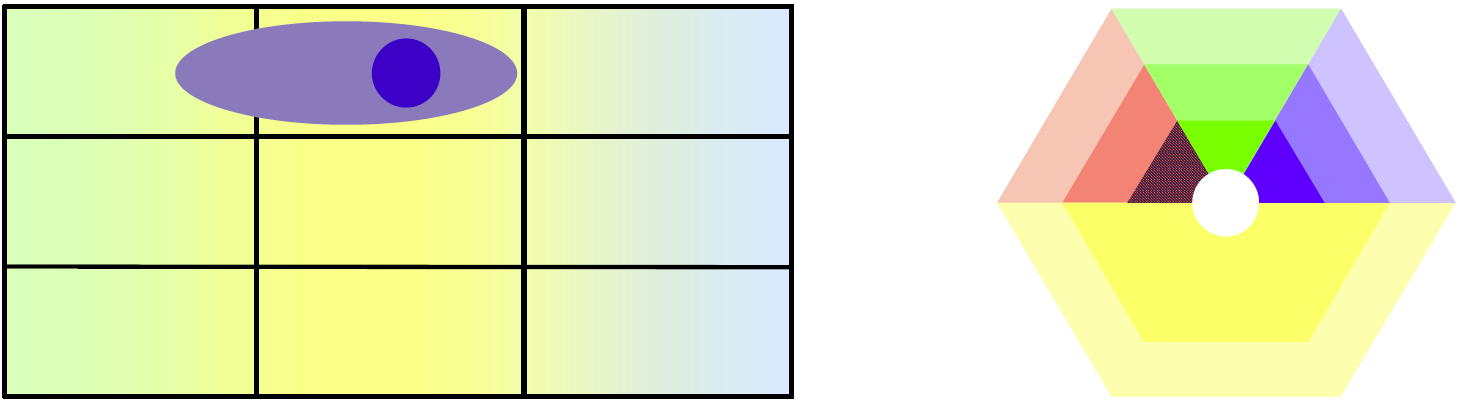
\includegraphics[scale=0.2]{figuras/17}
  	\captionsetup{width=.95\textwidth}
  	\caption{Posición del punto de vista proceso de negocio conceptualmente y marco del punto de vista \cite{ref9}}
  	\label{figura17}
  \end{figure}
  
  \subsection{Metamodelo\index{Metamodelo}}
  La Figura \ref{metamodelo4} se aprecia que el proceso de negocio tiene que ver con un rol o conjunto de roles, el proceso de negocio es disparado por un evento y el proceso de negocio genera un evento o un proceso de eventos, los procesos no son máquinas infinitas todo proceso es
  iniciado por uno o un conjunto de eventos.
  
  Los procesos generan objetos de negocio que es la representación del trabajo en la organización,  el servicio de negocio es lo que el proceso de negocio lleva a cabo estableciéndose entre los dos una relación de realización, el servicio es el core de negocio lo que el cliente mira, el proceso de negocio es lo que implementa realiza, materializa el servicio y el proceso de negocio funciona porque existen unos roles que se encargan de realizar el proceso. \cite{ref9}
  
  \begin{figure}[H]
  	\centering
  	\includegraphics{metamodelos/4}
  	\captionsetup{width=.95\textwidth}
  	\caption{Metamodelo\index{Metamodelo} Punto de Vista Proceso\index{Proceso} de Negocio\index{Negocio} \cite{ref9}}
  	\label{metamodelo4}
  \end{figure}
  
  \subsection{Modelo mInstituto}
  En esta vista se evidencian los procesos que se deben alinear para obtener un producto con un mayor valor agregado, para Creatics, se identifican los procesos de recepción de solicitud, firma del contrato, recepción y/o confirmación del pago y por último la generación de la licencia de uso y acceso a la plataforma.
  
  \begin{figure}[H]
  	\centering
  	\includegraphics[scale=0.7]{modelos/4}
  	\captionsetup{width=.95\textwidth}
  	\caption{Modelo Punto de Vista Proceso\index{Proceso} de Negocio\index{Negocio}: minstituto}
  	\label{modelo4}
  \end{figure}
  
  %aquí
  \section{Punto de Vista Cooperación\index{Cooperación} de Proceso\index{Proceso} de Negocio\index{Negocio}}
  El punto de vista de cooperación de proceso de negocio es usado para mostrar las relaciones
  de uno o mas procesos de negocio con los demás procesos de negocio y / o con su ambiente. Puede ser usado tanto para crear un diseño de alto nivel de procesos de negocio dentro de su contexto como para proveer un responsable administrador operacional para uno o mas de tales procesos con mando en sus dependencias. \cite{ref9}
  
  \begin{table}[H]
  	\centering
  	\begin{tabular}{p{3.7cm}p{8cm}}
  		\hline
  		\rowcolor[HTML]{0073a1}
  		{\color[HTML]{FFFFFF} \textbf{Nombre}} & {\color[HTML]{FFFFFF} \textbf{Cooperación\index{Cooperación} de Proceso\index{Proceso} de Negocio\index{Negocio}}} \\
  		\hline
  		\textbf{Stakeholder\index{Stakeholder}s} & Proceso\index{Proceso}s, Arquitectos de domino, Gerentes de Operaciones \\
  		\textbf{Preocupaciones} & Dependencias de los procesos de negocio, Responsabilidades \\
  		\textbf{Propósito} & Diseñar\index{Diseñar}, decidir \\
  		\textbf{Nivel de Abstracción\index{Abstracción}} & Coherencia\index{Coherencia} \\
  		\textbf{Capa} & Capa de Negocio\index{Negocio} (Aplicación\index{Aplicación}) \\
  		\textbf{Aspectos} & Comportamiento\index{Comportamiento}, (activo), (pasivo) \\
  		\bottomrule
  	\end{tabular}
  	\captionsetup{width=.95\textwidth}
  	\caption{Descripción punto de vista de cooperación de proceso \cite{ref9}}
  	\label{tabla8}
  \end{table}
  
  \begin{figure}[H]
  	\centering
  	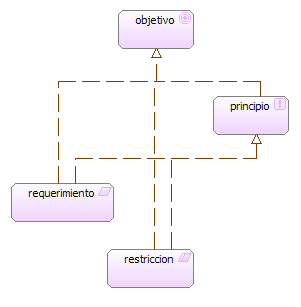
\includegraphics[scale=0.2]{figuras/18}
  	\captionsetup{width=.95\textwidth}
  	\caption{Posición del punto de vista de cooperación de proceso conceptualmente y marco del punto de vista \cite{ref9}}
  	\label{figura18}
  \end{figure}
  
  \subsection{Metamodelo\index{Metamodelo}}
  En la Figura \ref{metamodelo5} se ilustra el metamodelo perteneciente al punto de vista de cooperación de proceso el cual esta compuesto de los conceptos de los procesos del negocio y sus responsabilidades. En este punto de vista a al proceso se le asigna un rol, el rol se compone de interfaces, a la interface se le asigna interacciones y estas interacciones van a una capa de aplicación a través de una interface. \cite{ref9}
  
  \begin{figure}[H]
  	\centering
  	\includegraphics{metamodelos/5}
  	\captionsetup{width=.95\textwidth}
  	\caption{Metamodelo\index{Metamodelo} Punto de Vista de Producto\index{Producto} \cite{ref9}}
  	\label{metamodelo5}
  \end{figure}
  
  \subsection{Modelo mInstituto}
  En la vista se describe el soporte y razón de ser de Minstituto\index{Minstituto}.com que es generar soluciones tecnológicas aplicadas a la administración educativa, convirtiéndose en el objetivo estratégico de la organización. \\
  
  La plataforma web que corresponde a la ubicación del producto, es el medio que proporciona al cliente la confidencialidad, integridad y disponibilidad que su información y funciones de negocio necesitan. \\
  
  El acceso a la plataforma se establece a través de la generación de la licencia y en el contrato se determinan las diferentes características del producto, incluyendo actualizaciones y soporte especializado.
  
  \begin{figure}[H]
  	\centering
  	\includegraphics[scale=0.7]{modelos/5}
  	\captionsetup{width=.95\textwidth}
  	\caption{Modelo Punto de Vista de Producto\index{Producto}: minstituto}
  	\label{modelo5}
  \end{figure}
  
\section{Punto de Vista de Producto\index{Producto}}
Este punto de vista se describe como eje central el valor que uno o más productos ofrecen a la clientes u otras partes externas involucradas con la organización, muestra además la composición de uno o más productos en términos de cómo están compuestos, la asociación, el contrato y otros acuerdos. El punto de vista del producto se suele utilizar en el desarrollo de productos para diseñar un producto componiendo servicios existentes o mediante la identificación de nuevos servicios que se tienen que crear para este producto, dado el valor que un cliente espera de ella. \cite{ref9}

  \begin{table}[H]
  	\centering
  	\begin{tabular}{p{3.7cm}p{8cm}}
  		\hline
  		\rowcolor[HTML]{0073a1}
  		{\color[HTML]{FFFFFF} \textbf{Nombre}} & {\color[HTML]{FFFFFF} \textbf{Vista de Producto\index{Producto}}} \\
  		\hline
  		\textbf{Stakeholder\index{Stakeholder}s} & Diseñadores de producto, gerentes de producto, Arquitectos de proceso y de dominio \\
  		\textbf{Preocupaciones} & Desarrollo\index{Desarrollo} del producto y el valor que este ofrece a la organización \\
  		\textbf{Propósito} & Diseñar\index{Diseñar}, decidir \\
  		\textbf{Nivel de Abstracción\index{Abstracción}} & Coherencia\index{Coherencia} \\
  		\textbf{Capa} & Capa de Negocio\index{Negocio} (Aplicación\index{Aplicación}) \\
  		\textbf{Aspectos} & Comportamiento\index{Comportamiento}, información, (activo) \\
  		\bottomrule
  	\end{tabular}
	\captionsetup{width=.95\textwidth}
	\caption{Descripción Punto de Vista de Producto\index{Producto} \cite{ref9}}
	\label{tabla9}
  \end{table}

  \begin{figure}[H]
	\centering
	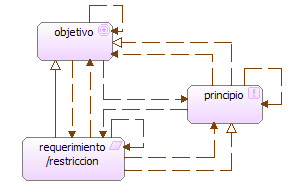
\includegraphics[scale=0.2]{figuras/19}
	\captionsetup{width=.95\textwidth}
	\caption{Posición del Punto de Vista de Producto\index{Producto} conceptualmente y marco del punto de vista \cite{ref9}}
	\label{figura19}
  \end{figure}
  
  \subsection{Metamodelo\index{Metamodelo}}
  La Figura \ref{metamodelo6} ilustra el punto de vista de producto el cual es la convergencia de los puntos de vista anteriores, es el esfuerzo por conocer la estructura, el esfuerzo por saber qué hace cada persona todo converge en el punto de vista que apunta al producto, el cual es un conjunto de servicios al cual se le adhiere un contrato y como elemento clave se le destaca un valor; el producto reposa sobre los procesos que son hechos por unos roles de negocio los cuales corresponden a unos actores. \cite{ref9}

  \begin{figure}[H]
	\centering
	\includegraphics{metamodelos/6}
	\captionsetup{width=.95\textwidth}
	\caption{Metamodelo\index{Metamodelo} Punto de Vista de Producto\index{Producto} \cite{ref9}}
	\label{metamodelo6}
  \end{figure}

  \subsection{Modelo mInstituto}
  El soporte y razón de ser de Minstituto\index{Minstituto}.com es generar soluciones tecnológicas aplicadas a la administración educativa, siendo la plataforma web el medio que proporciona al cliente la confidencialidad, integridad y disponibilidad que su información y funciones de negocio necesitan.  El acceso a la plataforma se establece a través de la generación de la licencia y en el contrato se determinan las diferentes características del producto, incluyendo actualizaciones y soporte especializado.

  \begin{figure}[H]
	\centering
	\includegraphics[scale=0.7]{modelos/6}
	\captionsetup{width=.95\textwidth}
	\caption{Modelo Punto de Vista de Producto\index{Producto}: minstituto}
	\label{modelo6}
  \end{figure}